\documentclass{rapportCS}
\usepackage{lipsum}
\title{Control Theory Report} %Titre du fichier

\begin{document}

%----------- Informations du rapport ---------

\logoentreprise{logos/parissaclay.png}

\titre{Speed Control of an Electrical Drive} % Title
\soustitre{Vitesse - Track A - Trinome 32}

\eleve{Jin DING \\
Carlos BENÍTEZ ROSETY \\
Marcos Ichiro SASAKI}

\infocours{TP Report \\ Control Theory}

\dates{19/09/2025 - 22/10/2025}

%----------- Initialisation -------------------
        
\fairemarges %Afficher les marges
\fairepagedegarde %Créer la page de garde

%----------- Abstract -------------------
\vspace*{\stretch{1}}
\begin{center}
	\begin{abstract}
        \lipsum[1-2]
    \end{abstract}
\end{center}
\vspace*{\stretch{1}}
\newpage

%------------ Table des matières ----------------

\tabledematieres % Créer la table de matières

%------------ Corps du rapport ----------------


%------------ Section 1 ----------------

\section{Identification of the System Parameters}

\subsection{Introduction}

The objective of this practical work is to design and implement control strategies for the speed regulation of a direct current (DC) electrical drive system. Such systems play a vital role in modern engineering applications, including transportation, robotics, and industrial automation, where precise and stable control is required to ensure efficiency and reliability.

The study combines theoretical modeling with experimental validation and is structured in three main stages. First, the electrical and mechanical parameters of the DC motor are identified experimentally using a platform composed of two coupled DC machines, sensors, and a DC/DC power converter. Second, controllers are designed and tested in simulation using Matlab/Simulink---an inner current loop designed by pole placement and an outer speed loop developed using a linear quadratic (LQ) approach. Finally, these controllers are implemented on the physical system to assess their real-time performance and compare experimental results with simulations.

The overarching goal is to analyze how different control structures and parameters influence the dynamic behavior of the system, and to demonstrate the practical application of modern control techniques in achieving stable and accurate speed regulation in electromechanical systems.

\subsection{Armature resistance and inductance: $R$ and $L$}


\subsection{Voltage constant and torque constant: $K_e = K_c$}


\subsection{Coulomb friction torque and viscous friction coefficient: $C_s$ and $f$}


\subsection{Moment of inertia of the system: $J$}





\newpage
%------------ Section 2 ----------------

\section{Controller Design and Validation by Simulations}
\lipsum[4-6]





\newpage
%------------ Section 3 ----------------

\section{Experimental Validation of the Controllers}

\label{sec:exp}

This section reports the laboratory validation of the controllers designed in Part~2. 
Several Simulink configurations were used successively (current loop, speed loop, and finally the observer). 
Due to limited laboratory time, \textbf{only the final implementation corresponding to the observer (Part~3.3) was saved as a representative Simulink diagram}. 
However, \textbf{all measurement results} obtained at each step were recorded and are presented below to assess the performance of every loop. 
Earlier configurations for the current and speed control followed the same structure as the final one (inner current loop, outer speed loop, voltage saturation, and acquisition blocks).

\vspace{4pt}
\noindent\textit{Practical constraints.} For hardware safety, the armature current was limited to 20~A, voltage commands were saturated at $\pm9$~V, and step amplitudes were increased gradually to avoid excessive mechanical stress and large current transients.

%-------------------- 3.1 --------------------
\subsection{Current Regulation Experiment}

The experimental results of the current control loop are shown in Figure~\ref{fig:exp_I_20A}. 
The upper plot displays the armature current (\textit{courant}) and the lower plot shows the corresponding motor speed (\textit{vitesse}). 
Several step changes were applied to the current reference, increasing successively from approximately 1~A to 2~A, 3~A and finally 10~A. 
The current follows the reference with a fast transient and negligible overshoot, demonstrating a well-tuned inner current loop. 
Small fluctuations in the measured signal are mainly due to sensor noise. 
The motor speed evolves consistently with the current variations, rising up to about 1000~rpm and then decreasing when the current is reduced or reversed. 
This confirms the expected electromechanical coupling between torque and speed. 
At the end of the experiment, both current and speed return smoothly to zero when the converter command is disabled.

\begin{figure}[H]
    \centering
    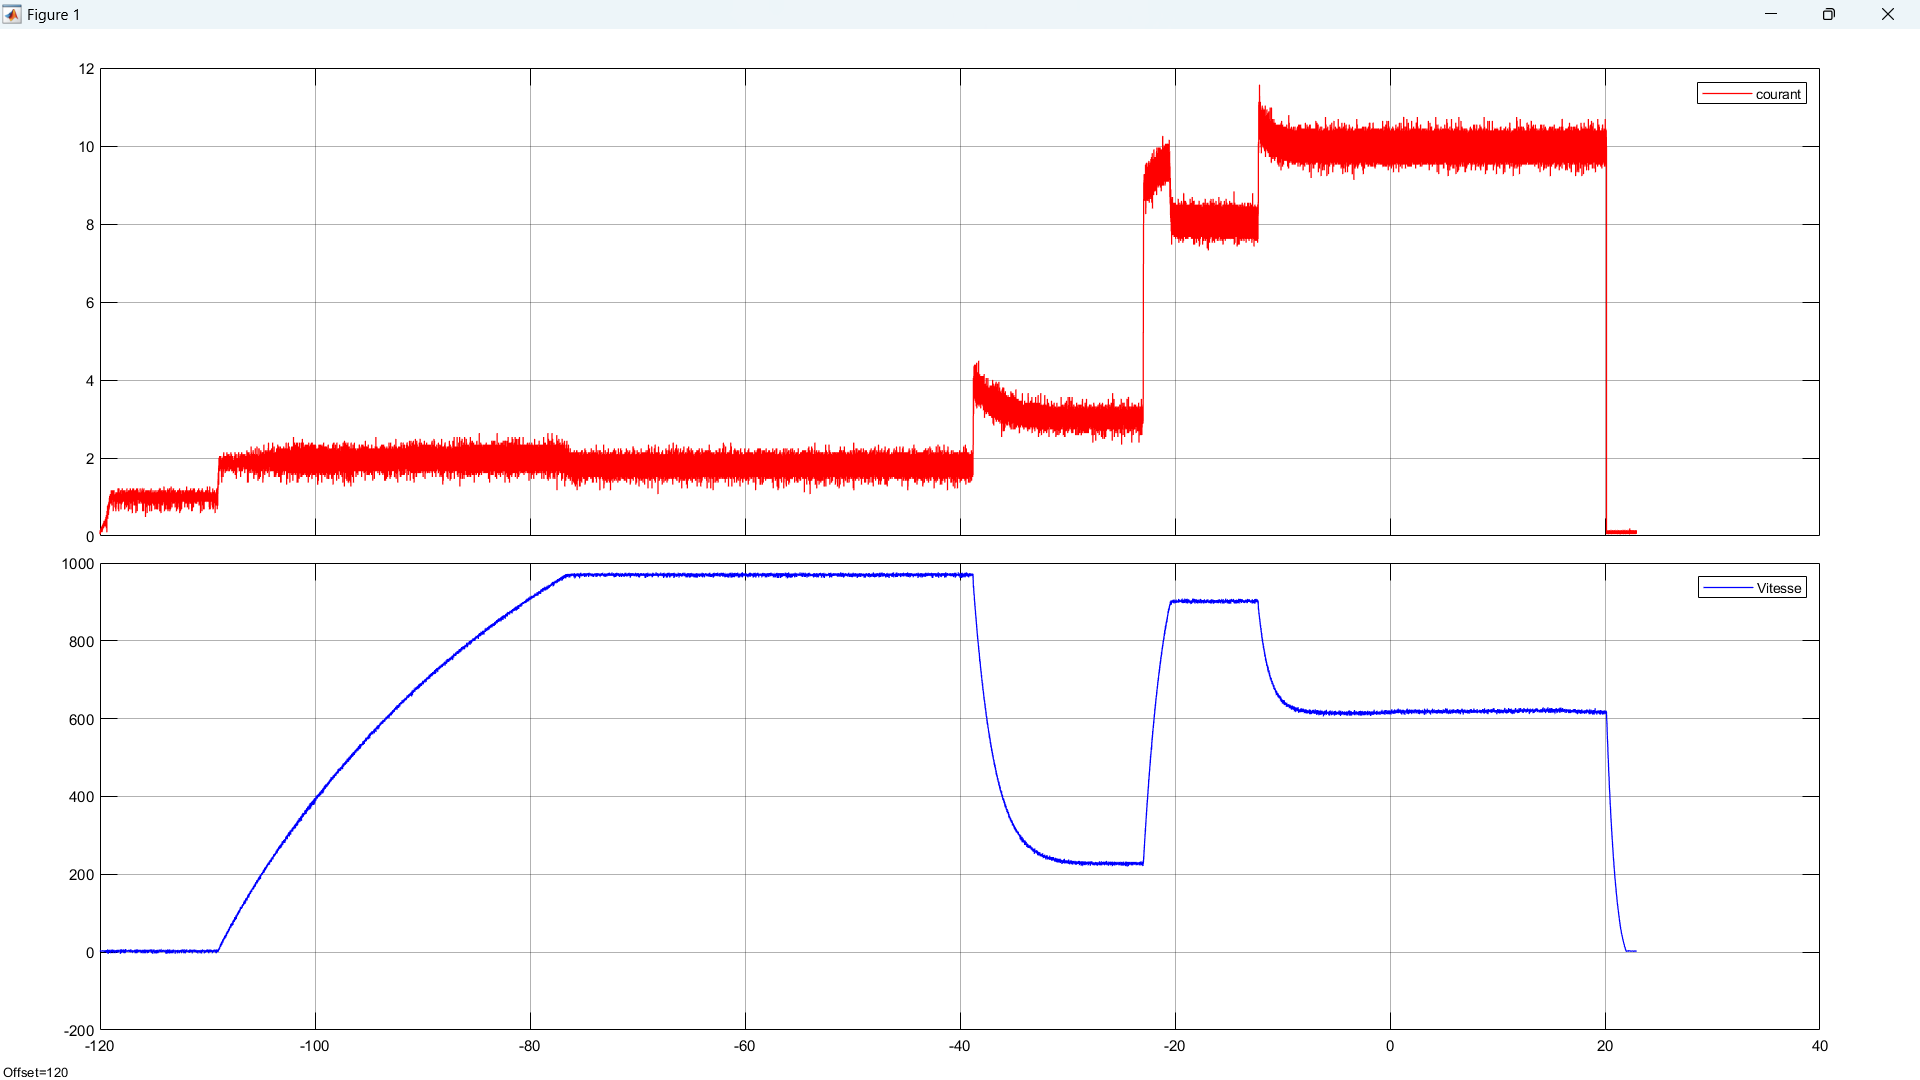
\includegraphics[width=\linewidth, keepaspectratio]{figures/PP1.png}
    \caption{Measured current (top, in~A) and speed (bottom, in~rpm) during the current regulation test. 
    The current loop shows fast and stable response with negligible overshoot.}
    \label{fig:exp_I_20A}
\end{figure}


%-------------------- 3.2 --------------------
\subsection{Speed Regulation Experiment}

The experimental validation of the speed controller was performed following the four test scenarios defined in Question~2.2.c. 
For each case, the converter operated in ``Automatic'' mode, and the speed reference $\Omega^*(t)$ was imposed through the control panel. 
The measured motor speed (\textit{vitesse}) and armature current (\textit{courant}) were recorded simultaneously.

\begin{itemize}
    \item $\mathbf{Case~1:}$ $C_r(t)=0$, $\Omega^*(t)$ changes from $0$ to $300~\text{rpm}$ at $t=1~\text{s}$.
    \item $\mathbf{Case~2:}$ $C_r(t)=0$, $\Omega^*(t)$ changes from $0$ to $500~\text{rpm}$ at $t=1~\text{s}$.
    \item $\mathbf{Case~3:}$ $C_r(t)=0$, $\Omega^*(t)$ changes from $0$ to $1200~\text{rpm}$ at $t=1~\text{s}$.
    \item $\mathbf{Case~4:}$ $\Omega^*(t)$ changes from $0$ to $300~\text{rpm}$ at $t=1~\text{s}$, while the resistant torque $C_r(t)$ increases from $0$ to $5~\text{Nm}$ at $t=10~\text{s}$.
\end{itemize}

The measured responses are summarized in Figures~\ref{fig:exp_W_300}--\ref{fig:exp_W_disturbance}. 
In all cases, the speed regulation shows a well-damped transient with limited overshoot and negligible steady-state error. 
For moderate speed commands (300~rpm and 500~rpm), the current peaks remain within the admissible range (below 20~A), confirming that the current limiter effectively constrains the torque demand. 
When the reference is increased to 1200~rpm, the system still converges but the transient becomes slower, illustrating the saturation effect of the voltage converter.

When a disturbance torque of 5~Nm is applied at $t=10~\text{s}$, a brief speed drop is observed, immediately compensated by the integral action of the speed controller. 
The steady-state speed returns to its nominal value within less than one second, demonstrating the robustness of the closed-loop regulation against load disturbances.

\begin{figure}[H]
    \centering
    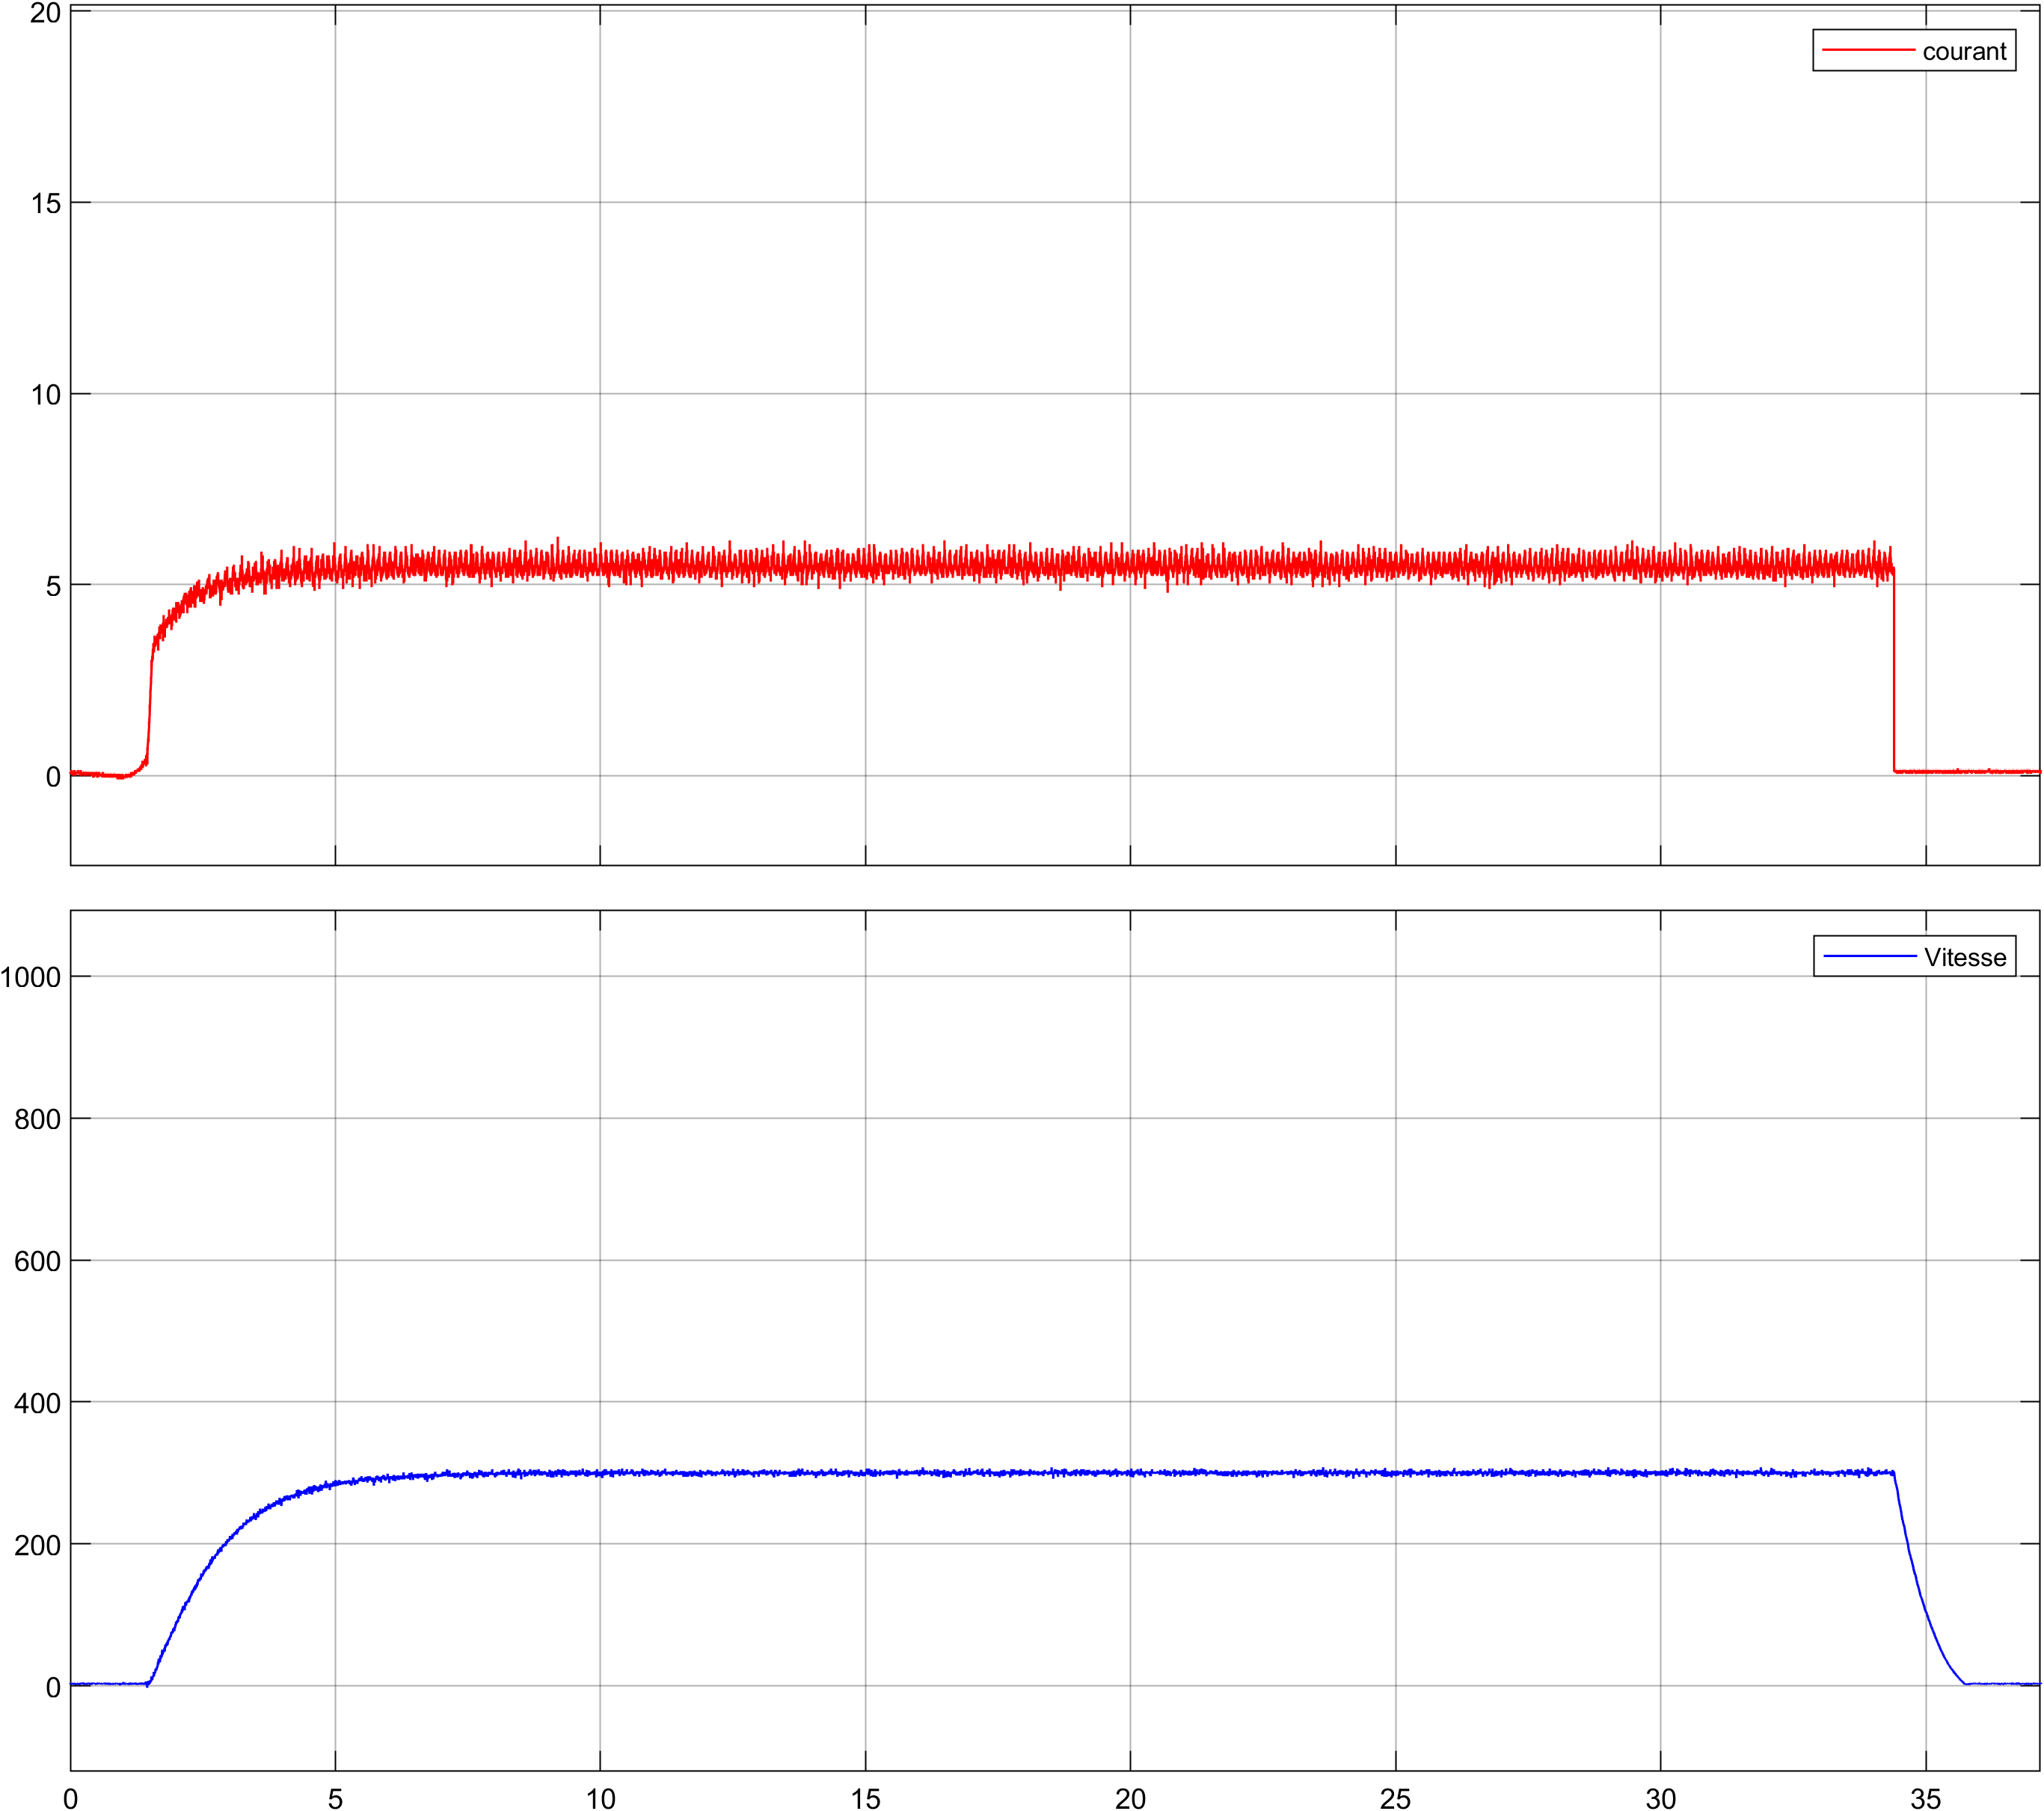
\includegraphics[width=\linewidth, keepaspectratio]{figures/p300.png}
    \caption{Speed loop --- measured response for a $0 \rightarrow 300~\text{rpm}$ reference step.}
    \label{fig:exp_W_300}
\end{figure}

\begin{figure}[H]
    \centering
    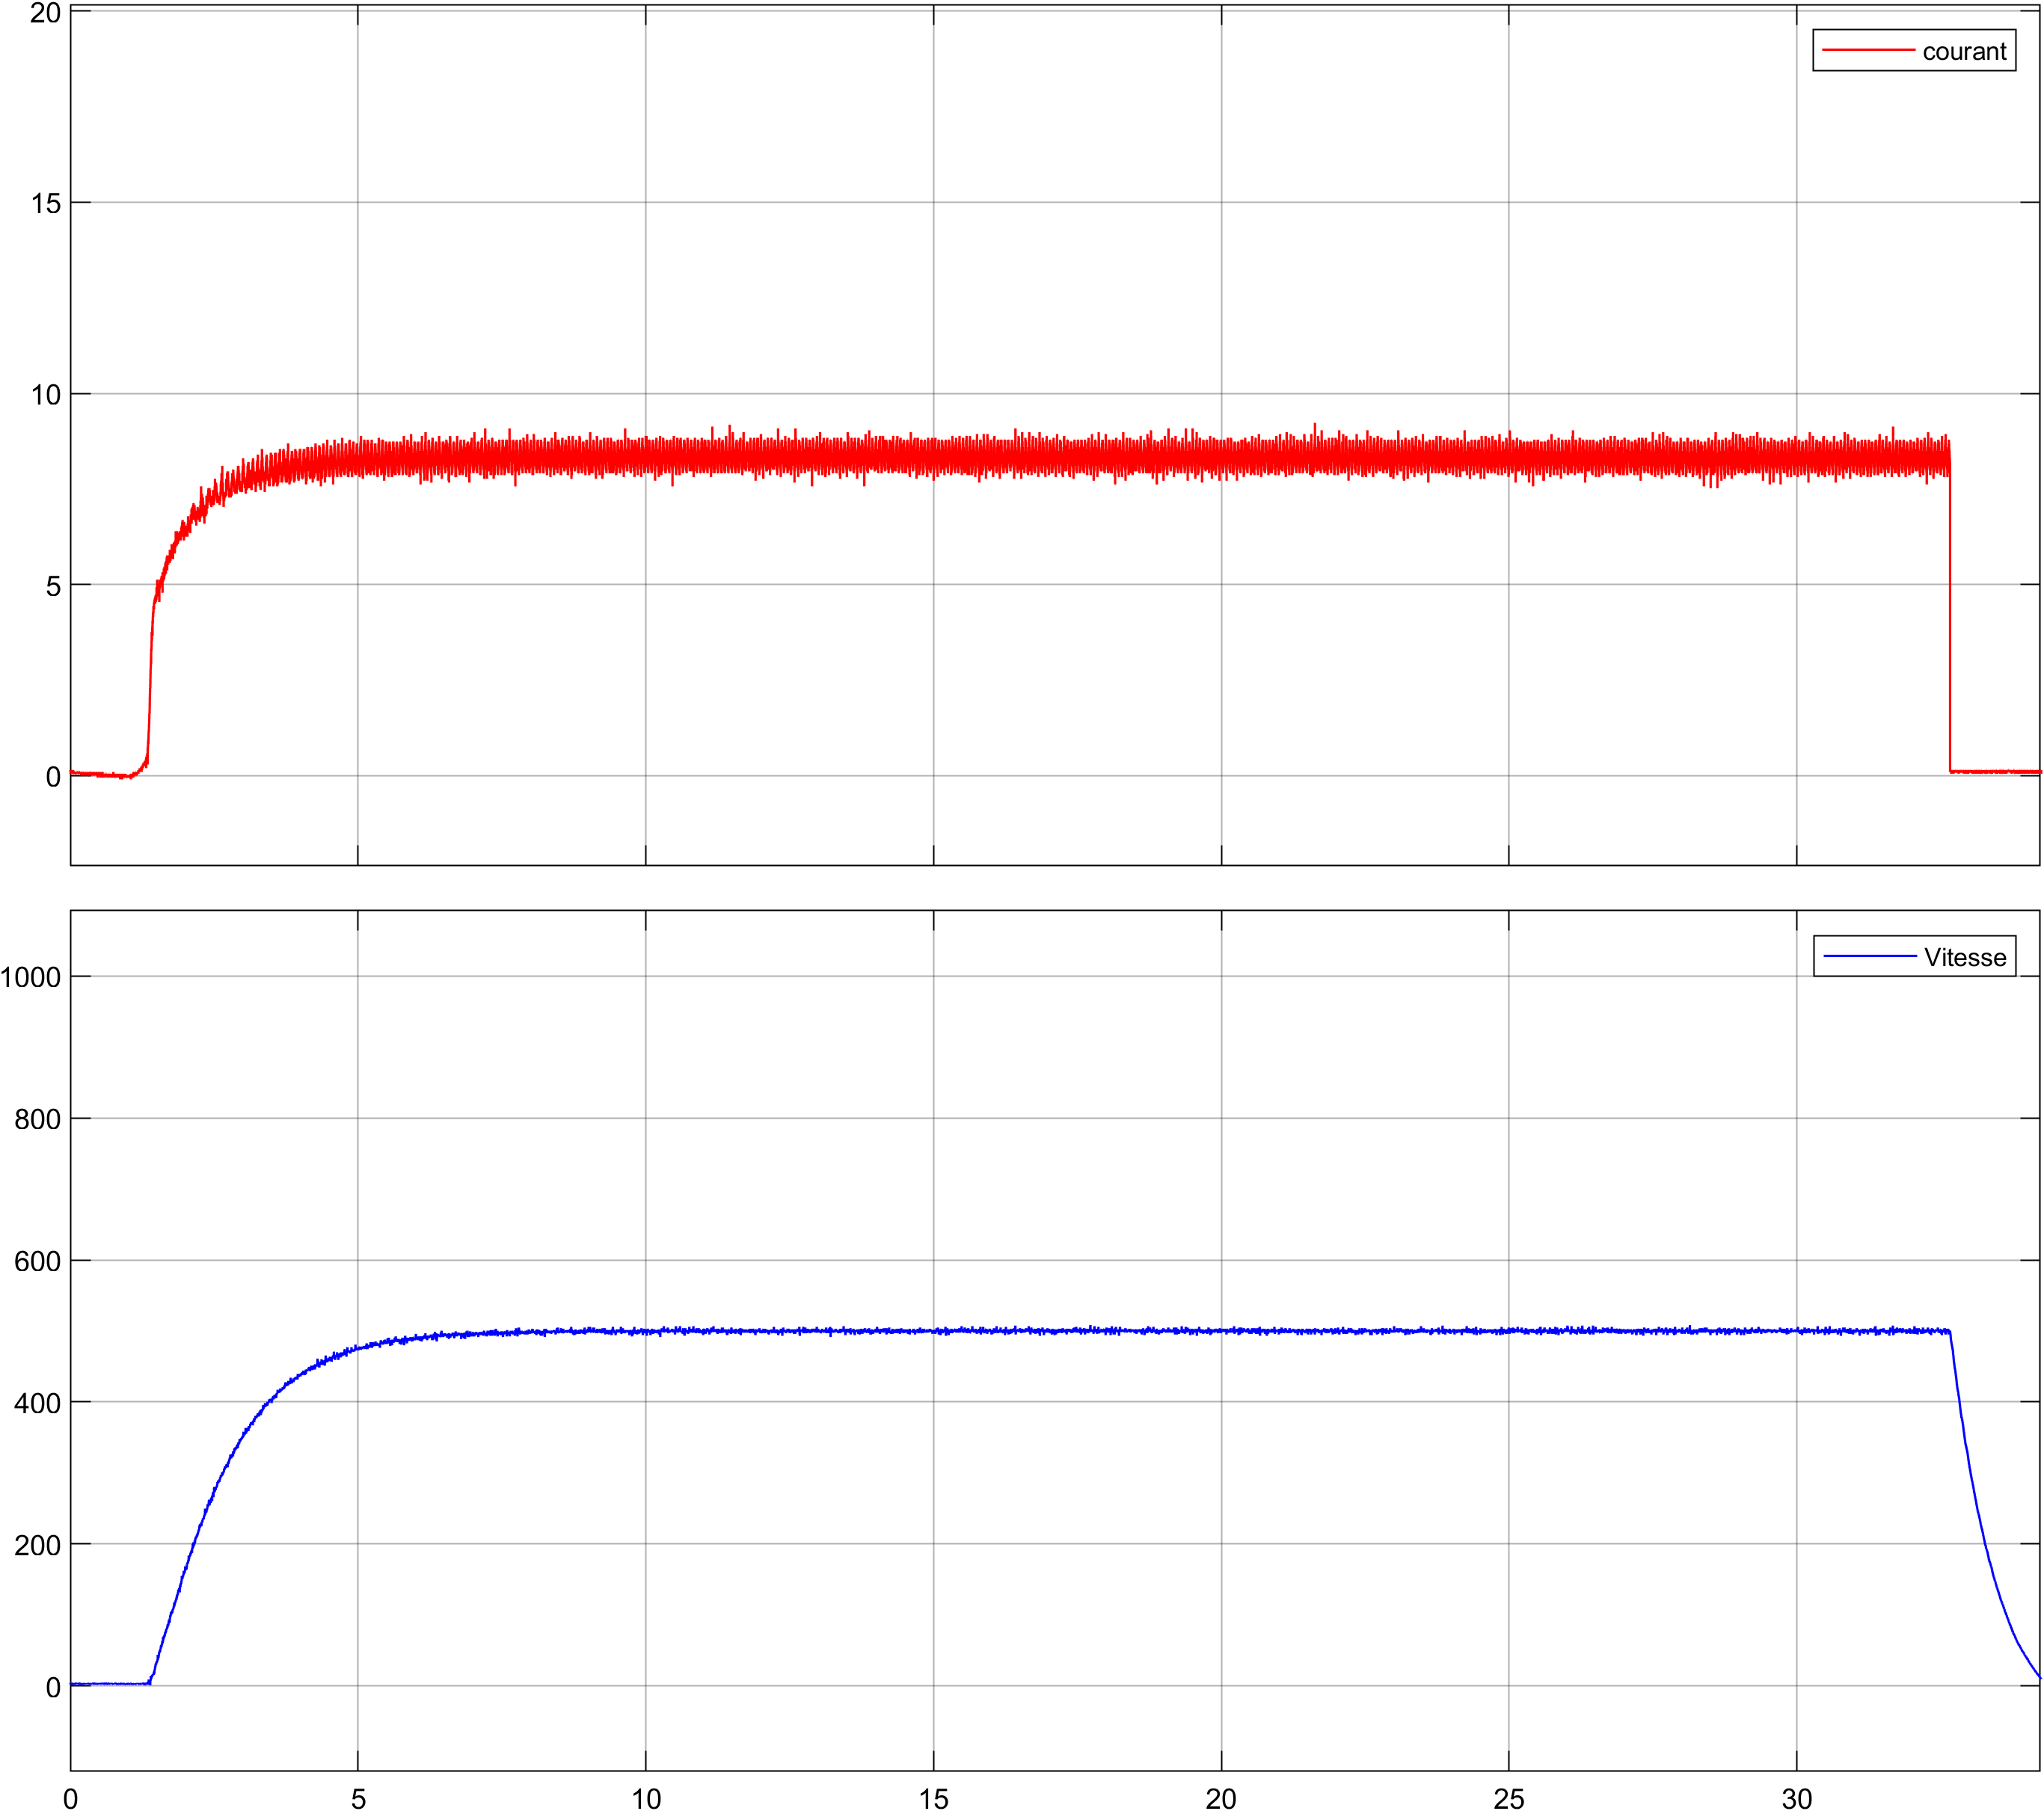
\includegraphics[width=\linewidth, keepaspectratio]{figures/p500.png}
    \caption{Speed loop --- measured response for a $0 \rightarrow 500~\text{rpm}$ reference step.}
    \label{fig:exp_W_500}
\end{figure}

\begin{figure}[H]
    \centering
    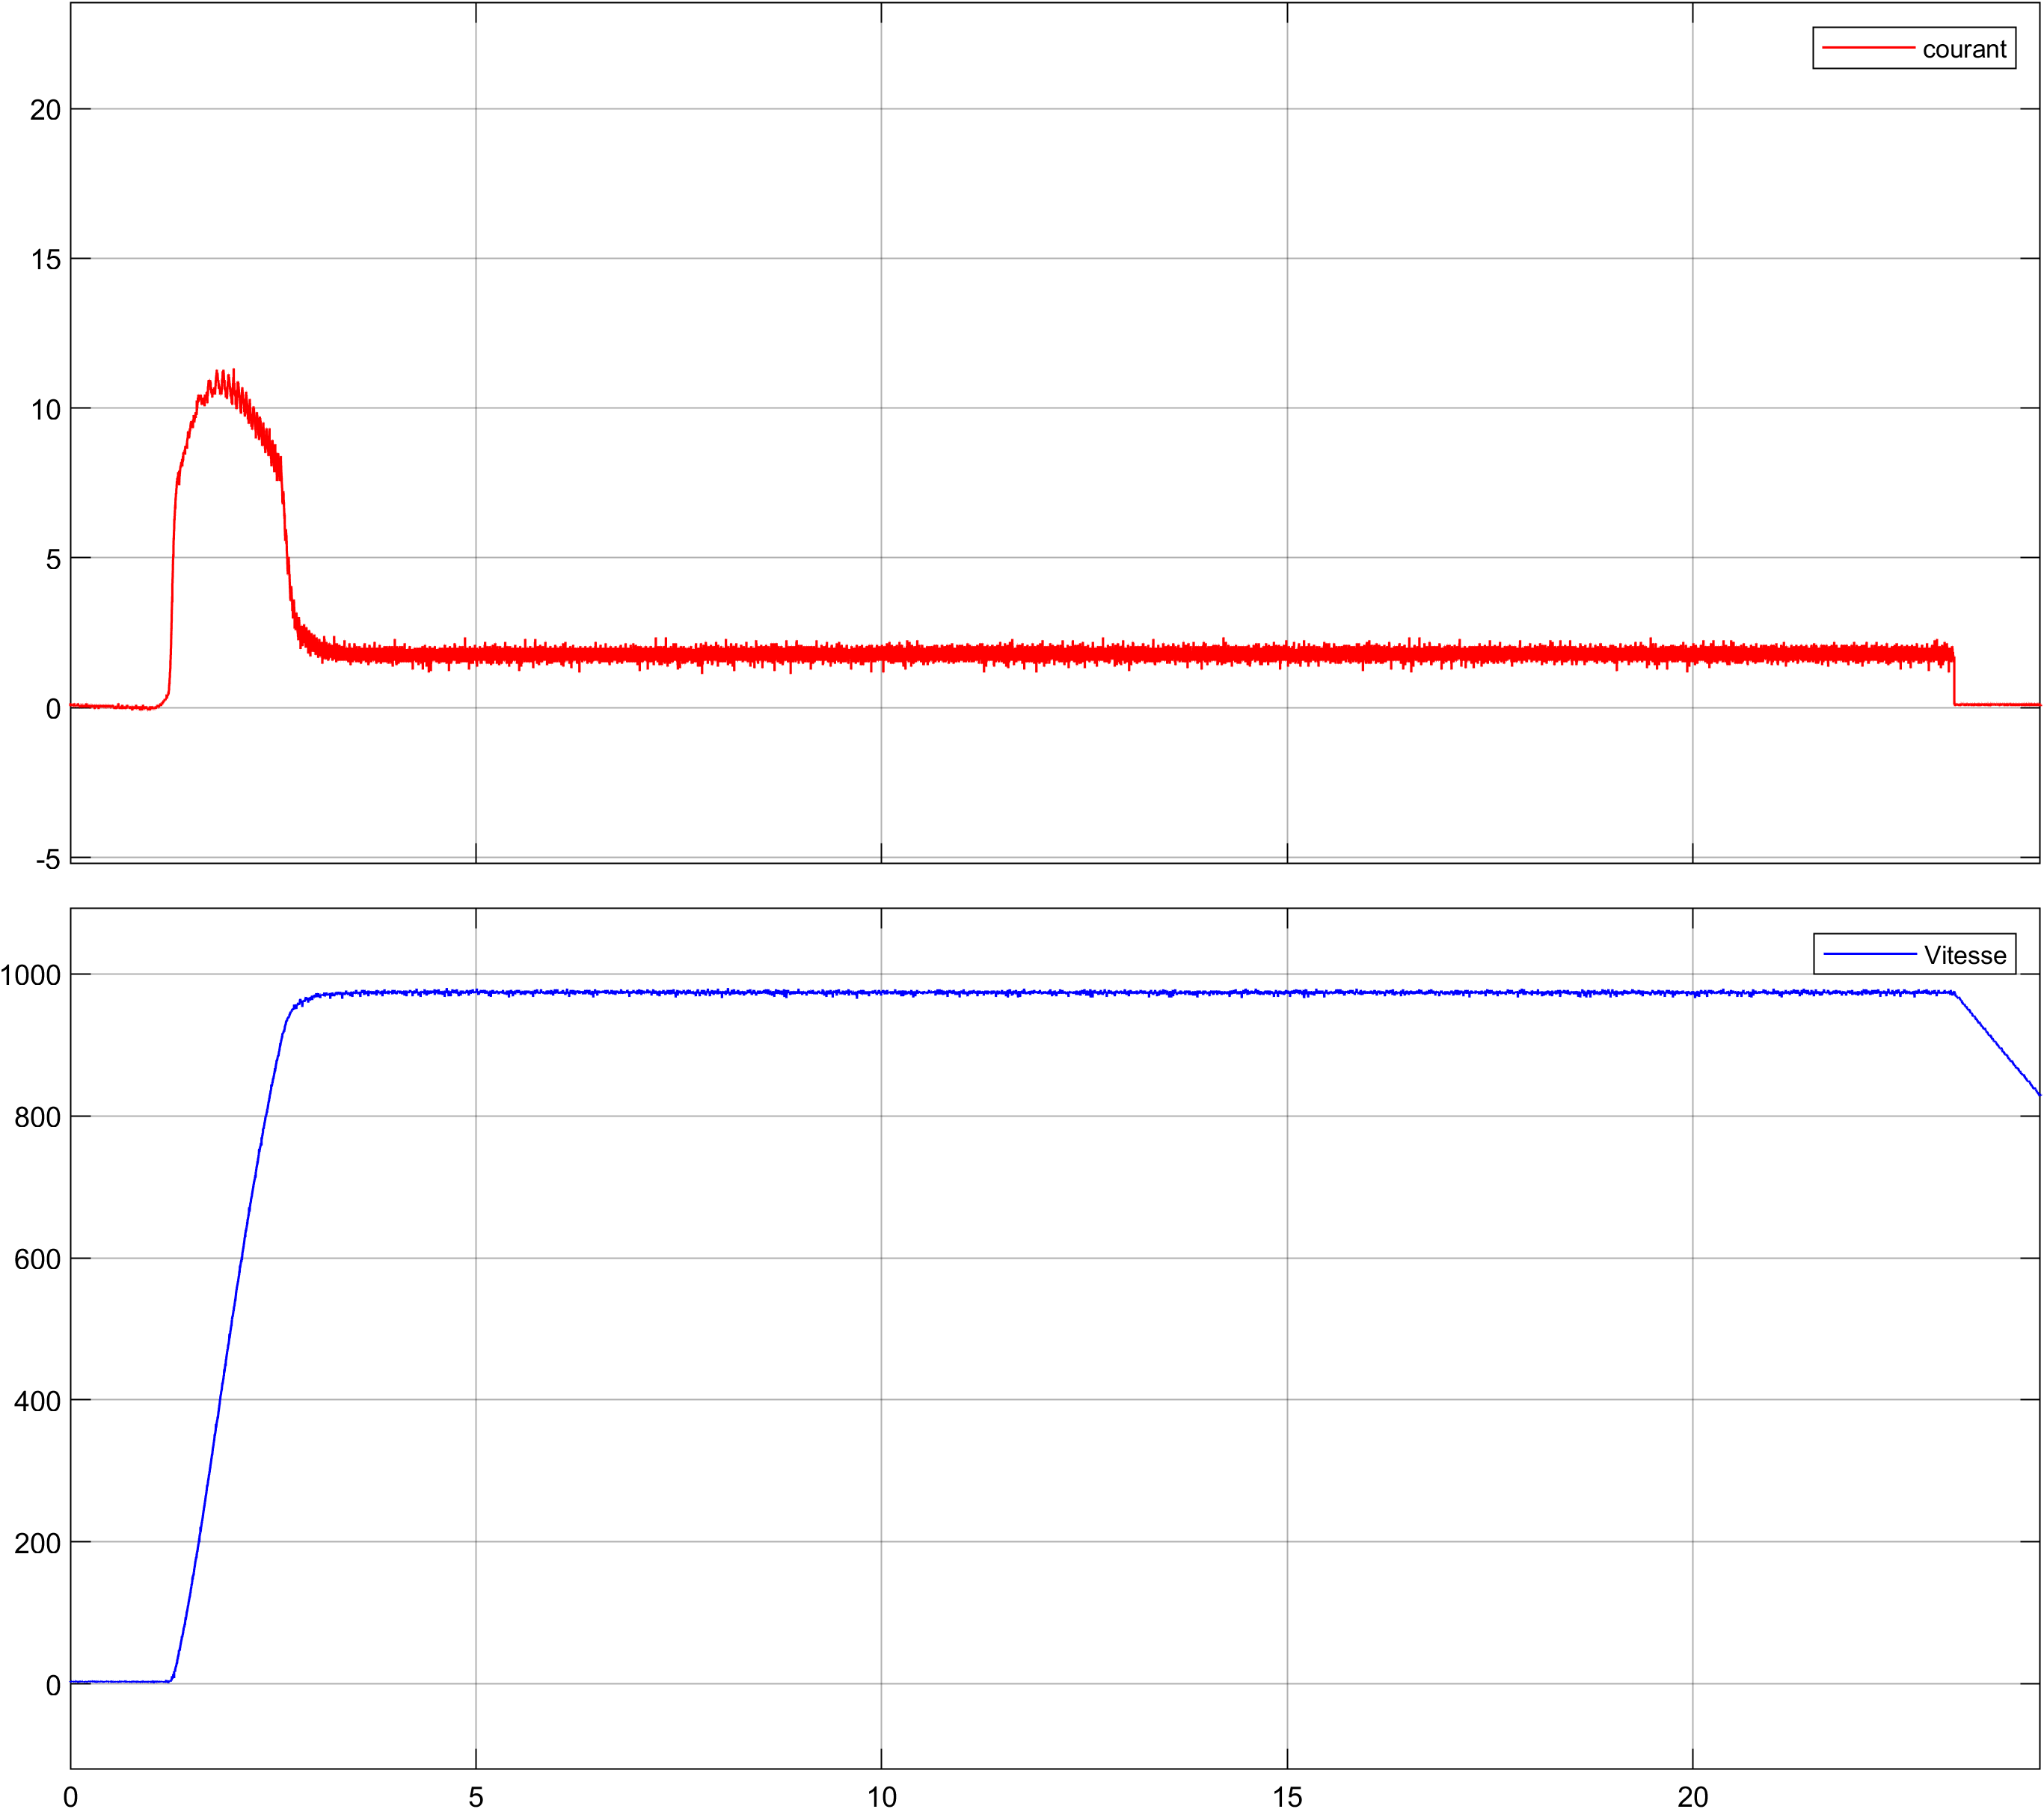
\includegraphics[width=\linewidth, keepaspectratio]{figures/p1200.png}
    \caption{Speed loop --- measured response for a $0 \rightarrow 1200~\text{rpm}$ reference step, showing converter saturation effects.}
    \label{fig:exp_W_1200}
\end{figure}

\begin{figure}[H]
    \centering
    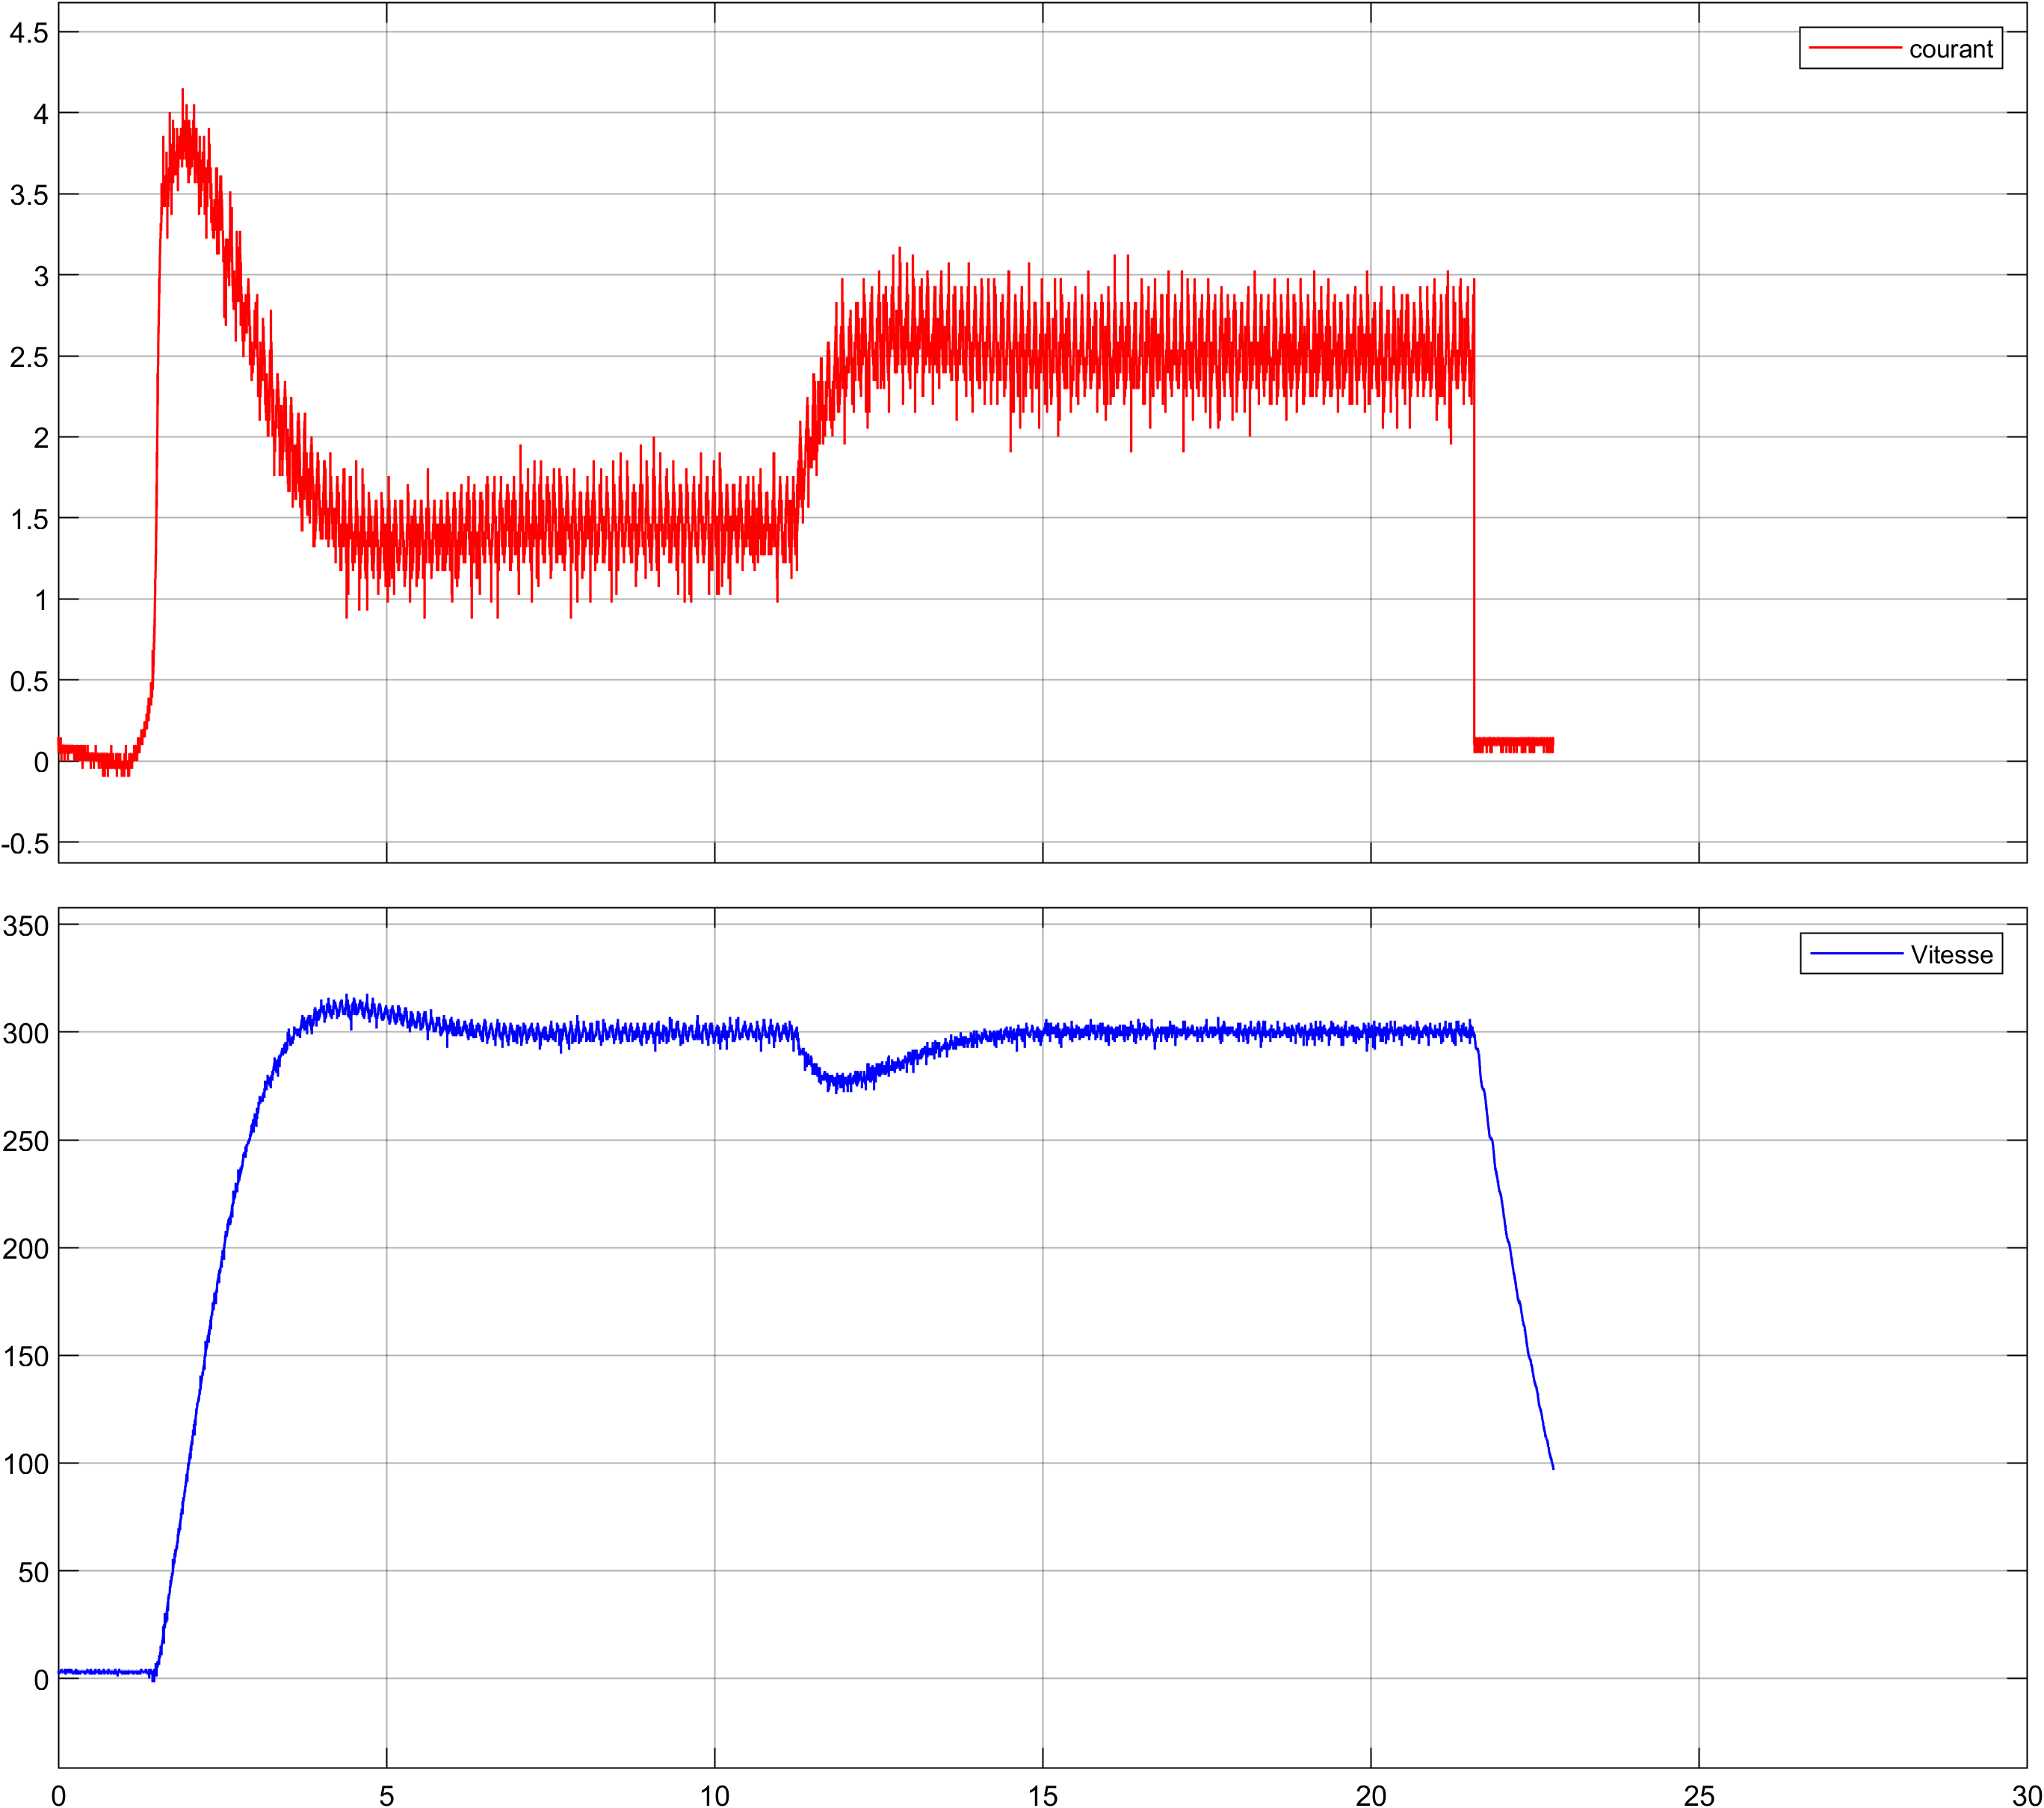
\includegraphics[width=\linewidth, keepaspectratio]{figures/p300cr5.png}
    \caption{Speed loop --- disturbance rejection test: a $5~\text{Nm}$ torque is applied at $t=10~\text{s}$. 
    The controller compensates the perturbation and restores the nominal speed.}
    \label{fig:exp_W_disturbance}
\end{figure}

%-------------------- 3.3 --------------------
\subsection{Observer Implementation and Validation}
\label{subsec:exp_obs}

Finally, the observer developed in Section~2.3 was implemented to estimate the states $[\hat I,\ \hat\Omega,\ \hat C_r]$. 
The \textbf{final Simulink configuration} used for all experiments is shown in Figure~\ref{fig:exp_obs_model}; it summarizes the complete control architecture (inner current loop, outer speed loop, observer, saturation, and I/O blocks).

\begin{figure}[H]
    \centering
    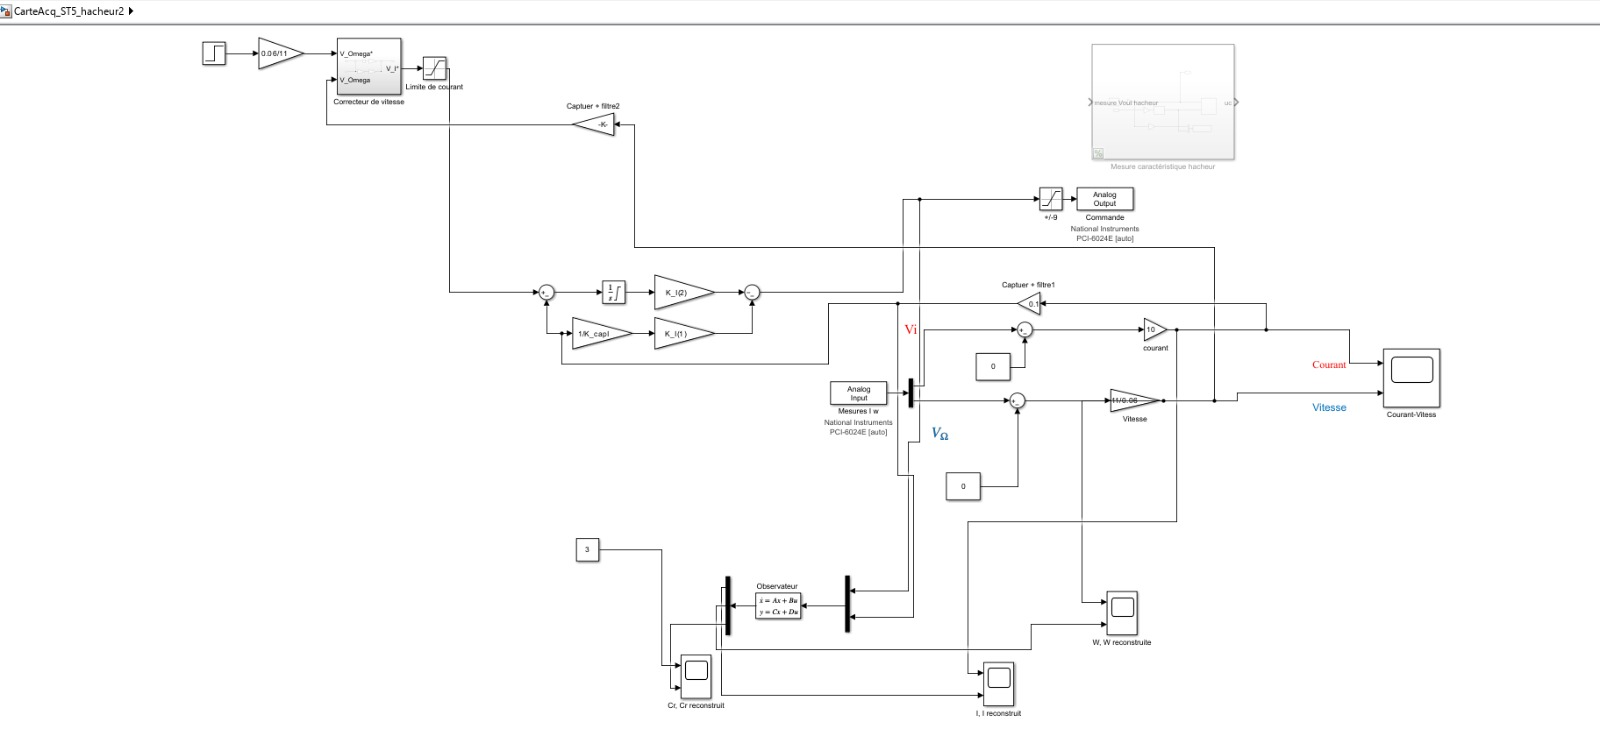
\includegraphics[width=\linewidth, keepaspectratio]{figures/simulink.png}
    \caption{Final Simulink implementation used on the bench (saved during Part~3.3). 
    Earlier configurations for the current and speed loops followed the same structure.}
    \label{fig:exp_obs_model}
\end{figure}

The current estimate converged rapidly and accurately. 
The speed estimate showed small mismatches and high-frequency noise, mainly due to sensor noise and converter nonlinearities. 
When using $\hat C_r$ for proportional disturbance compensation, the closed loop became sensitive to this noise and could lose stability. 
Therefore, compensation based on $\hat C_r$ was not retained on the bench without additional filtering or gain scheduling. 
Figure~\ref{fig:exp_obs_results} illustrates the convergence of the estimated variables towards their measured counterparts.

\begin{figure}[H]
    \centering
    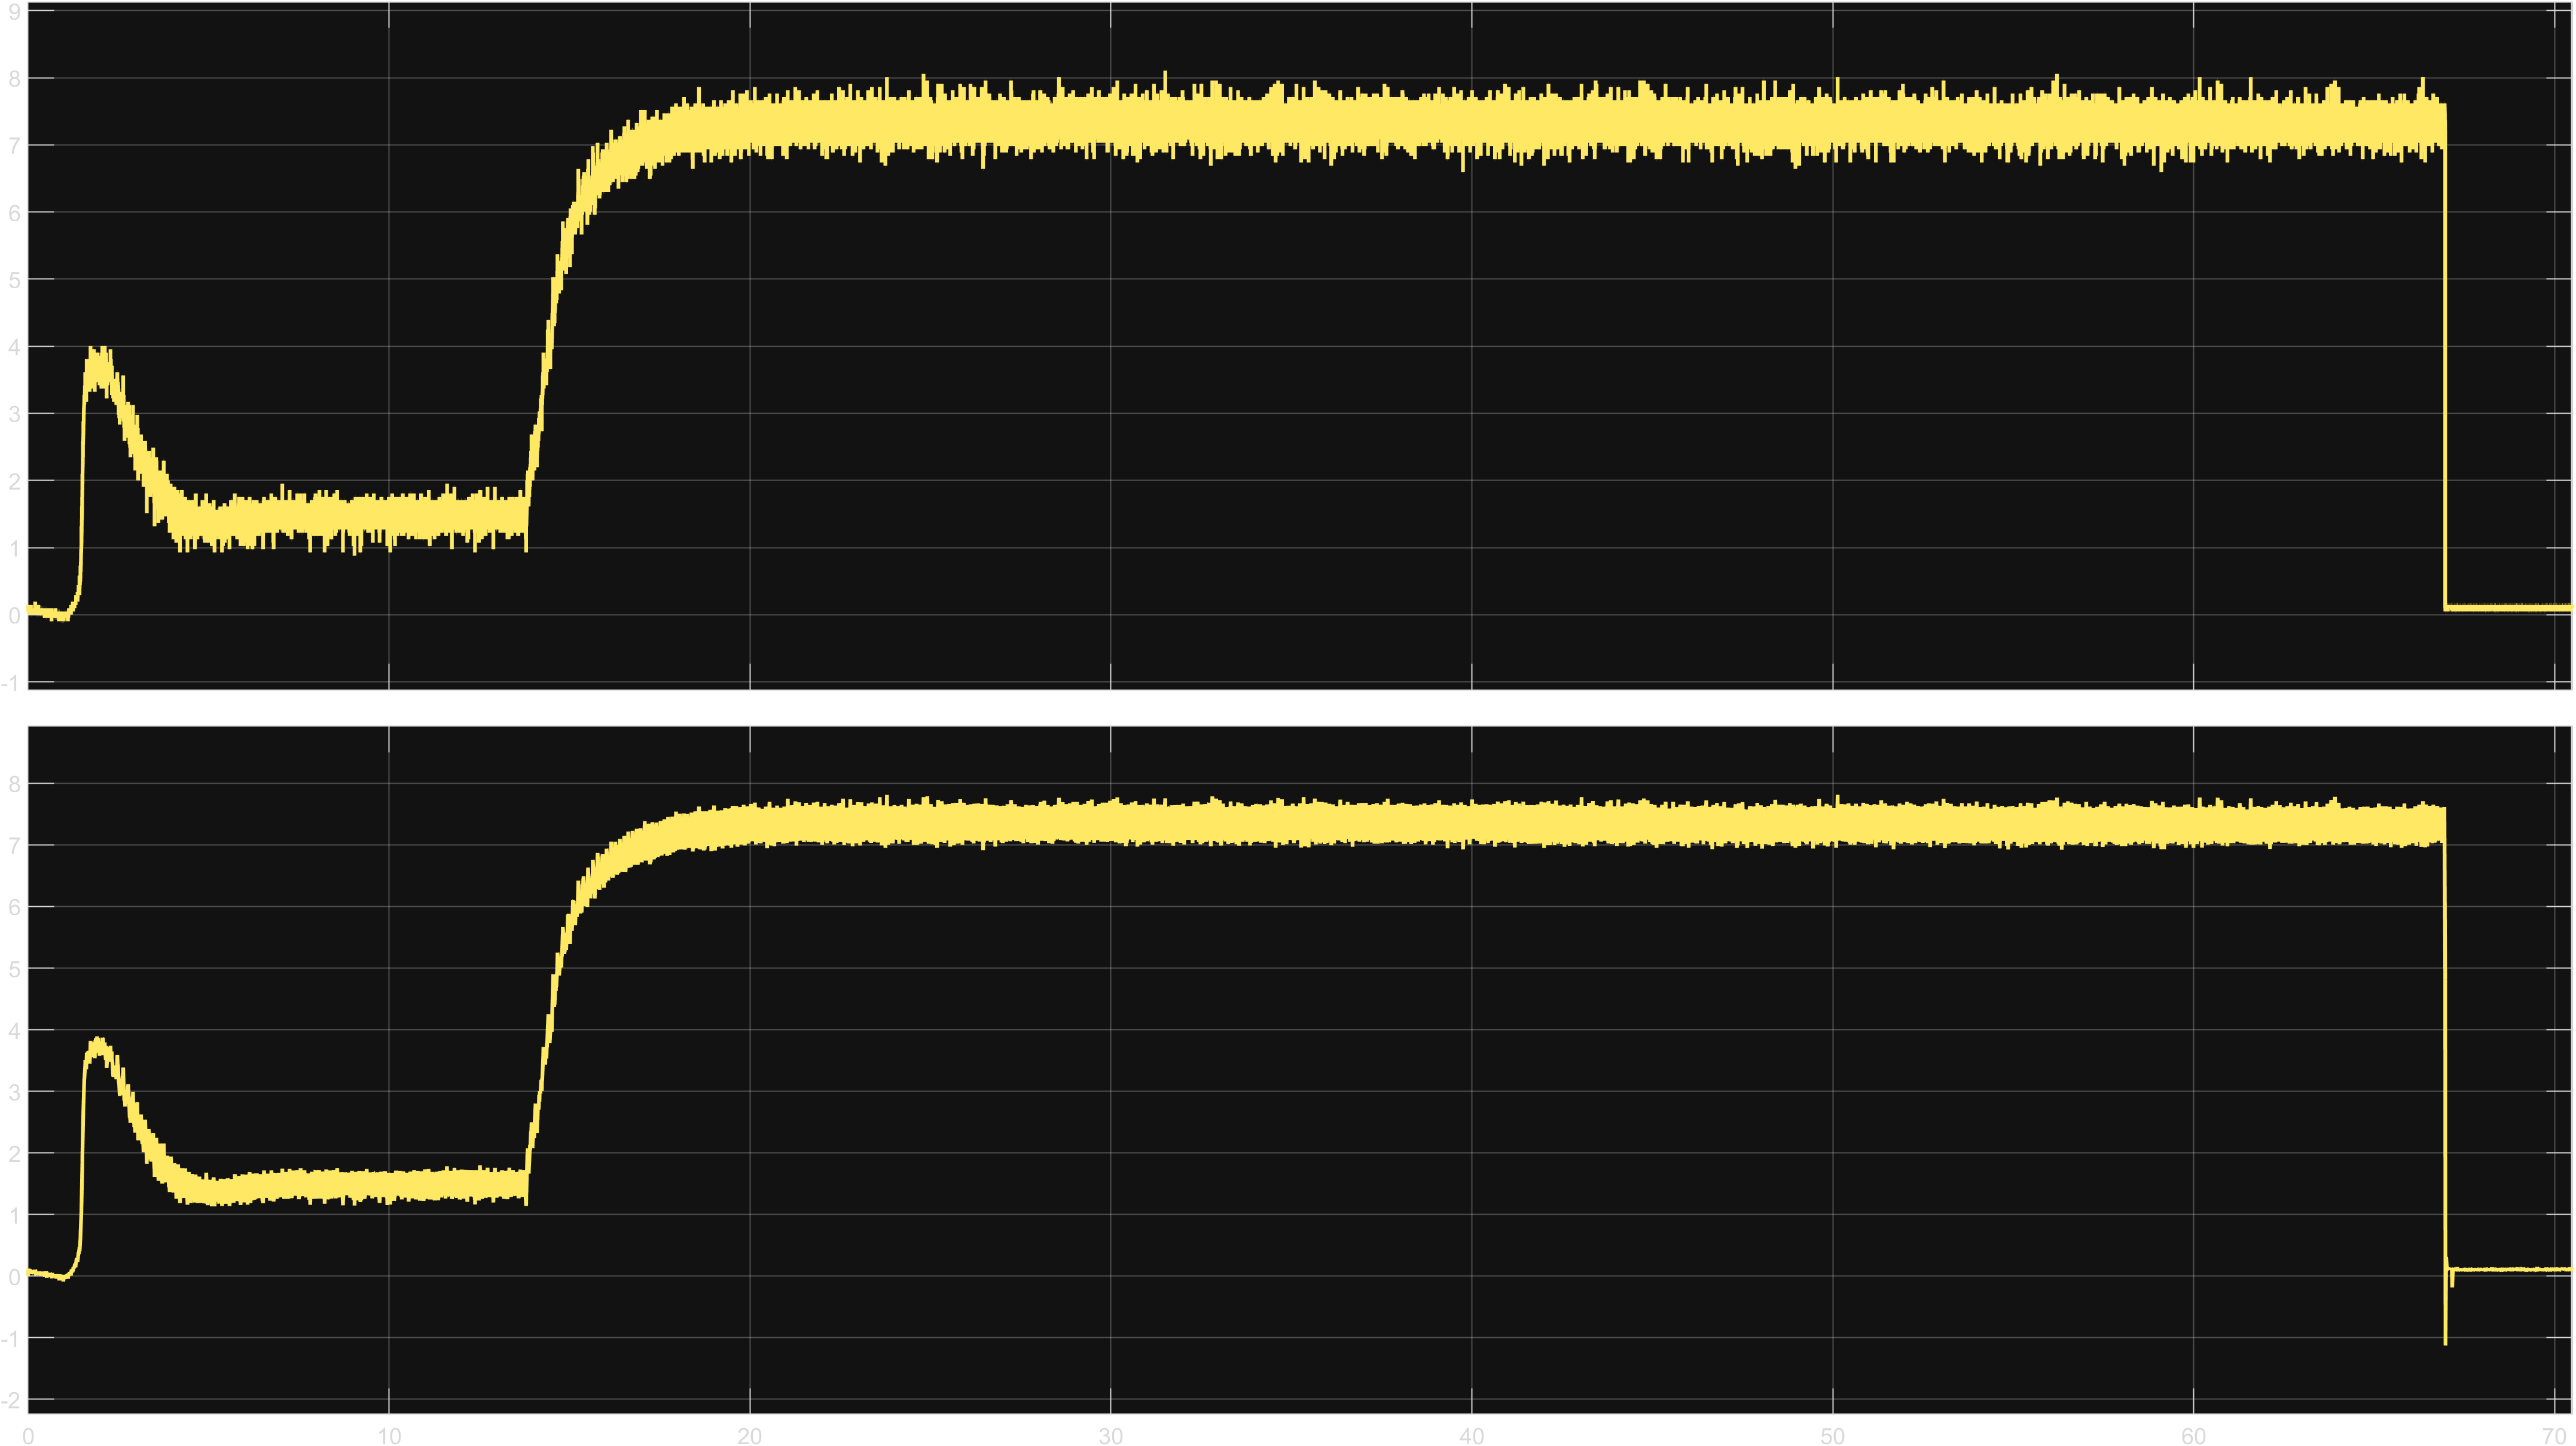
\includegraphics[width=\linewidth, keepaspectratio]{figures/p3i.png}
    \vspace{0.5em}
    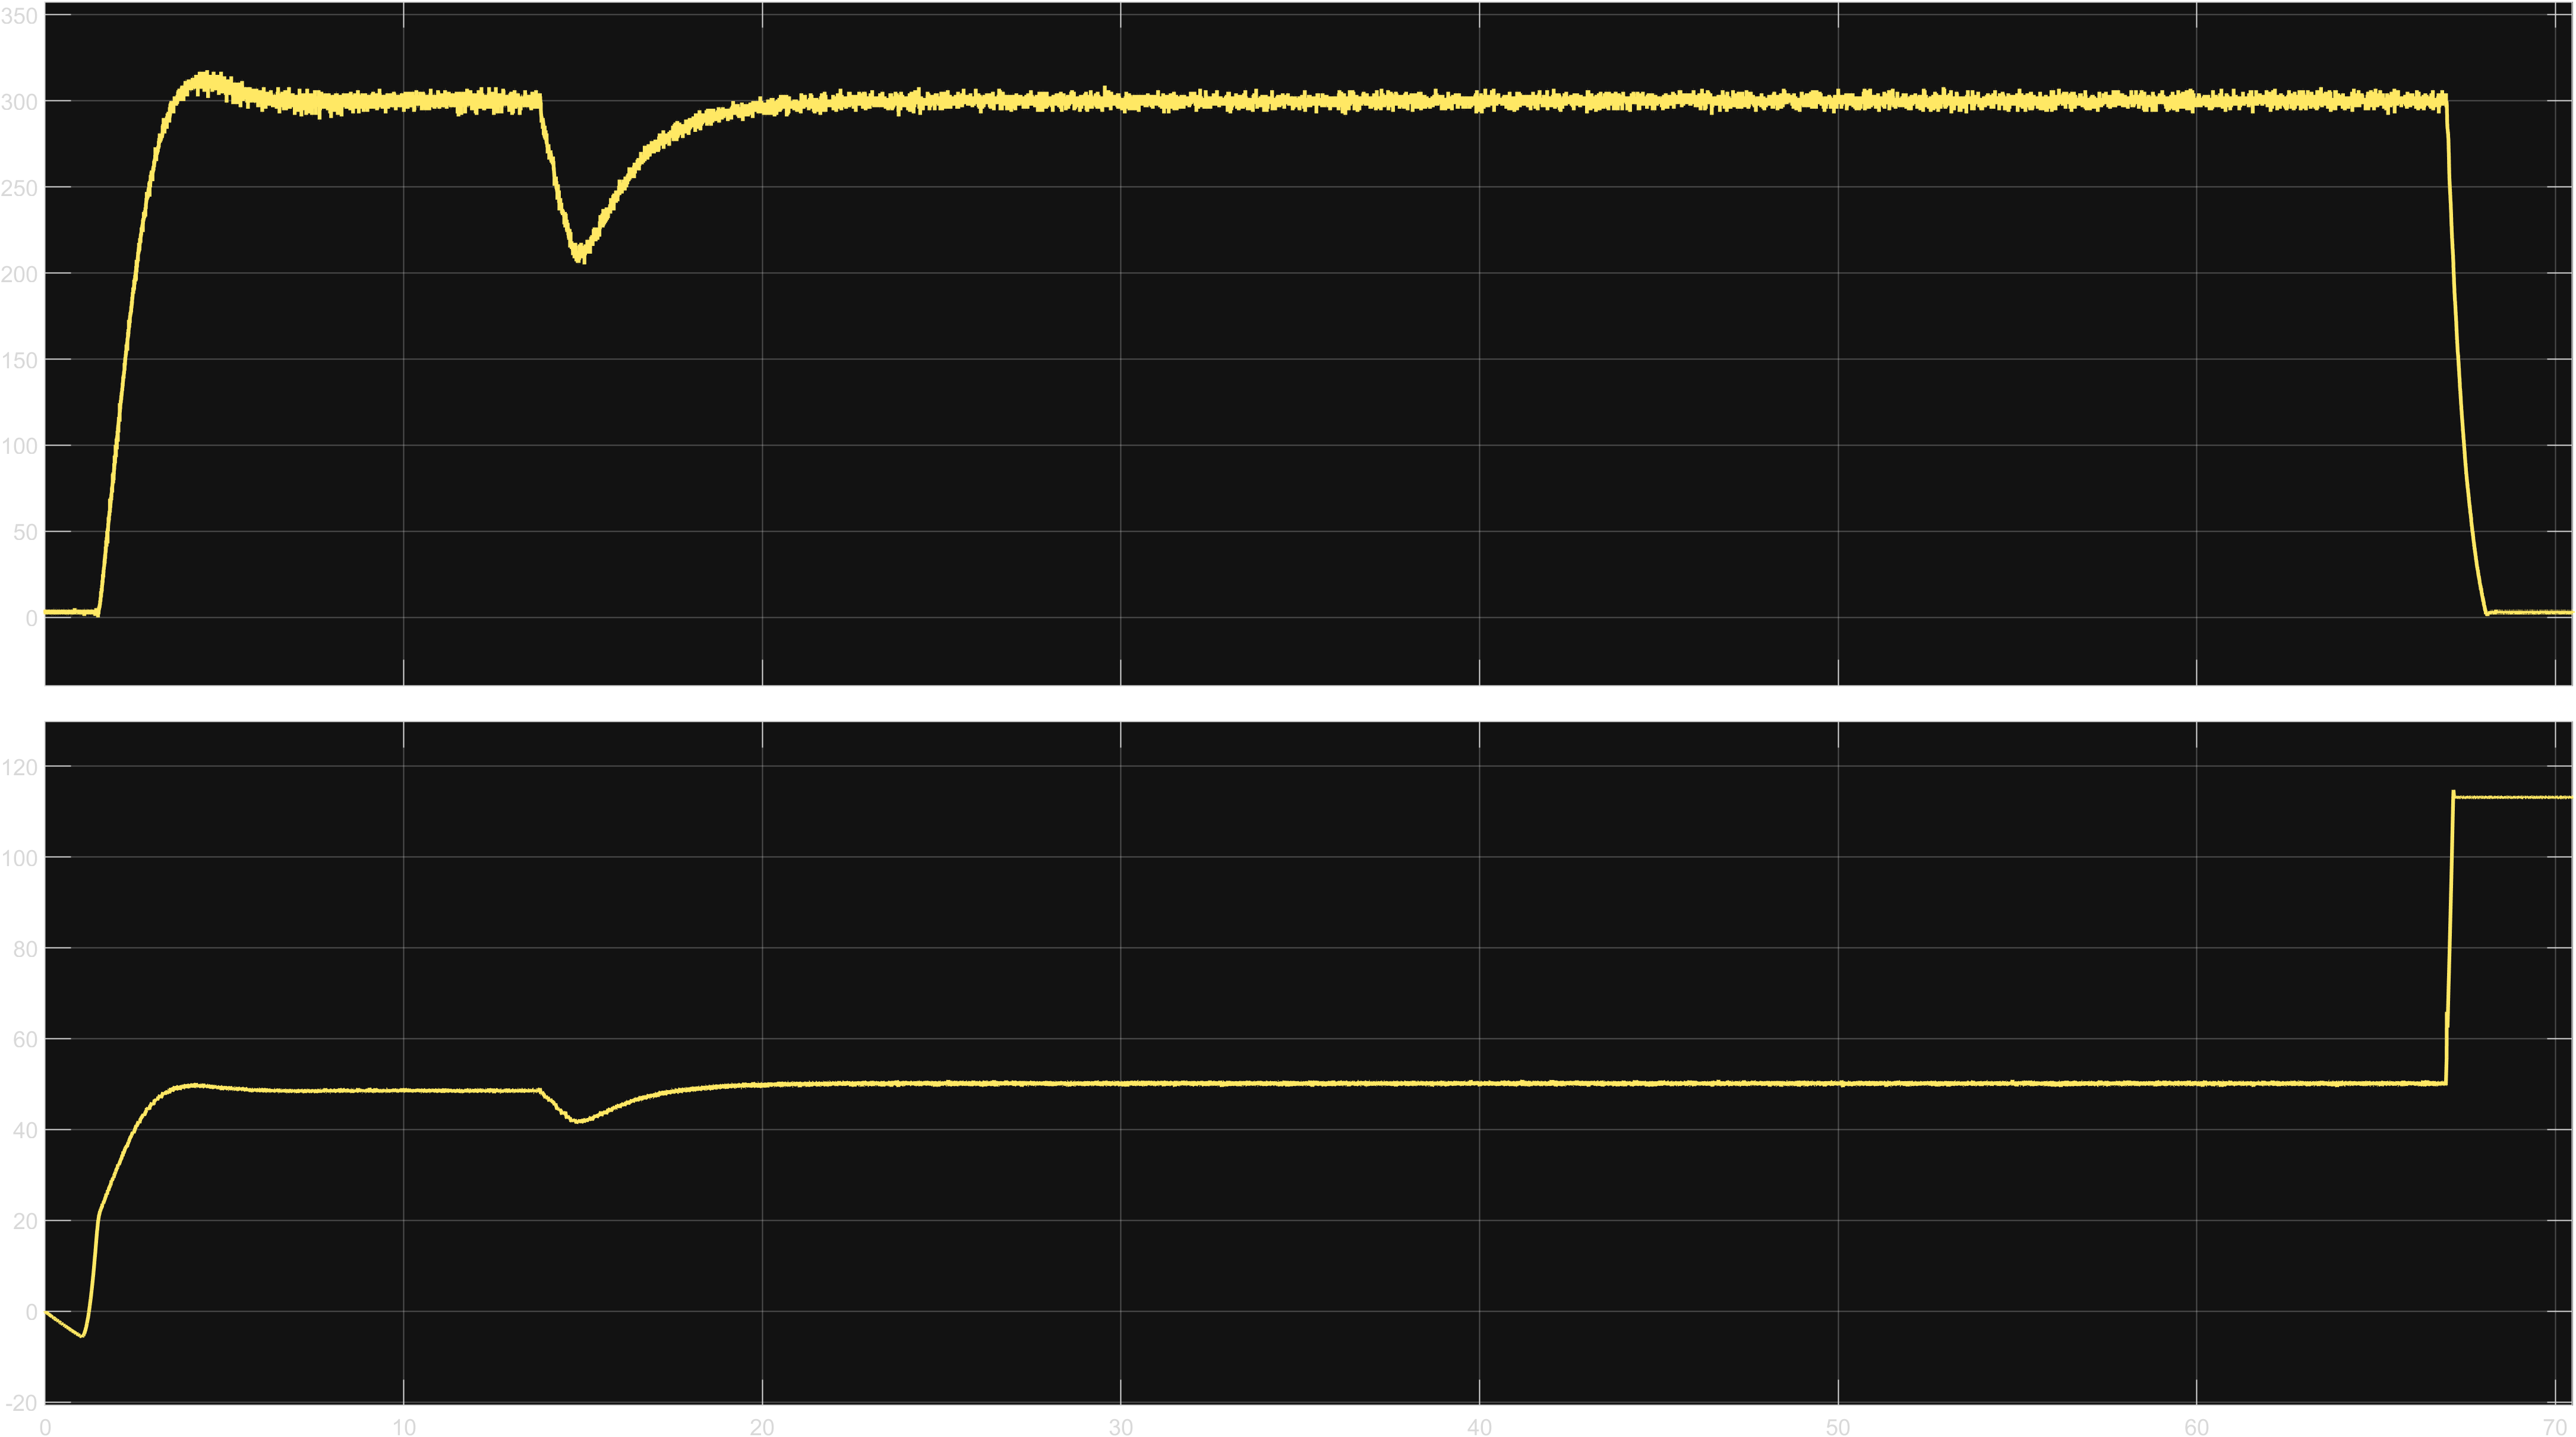
\includegraphics[width=\linewidth, keepaspectratio]{figures/pw.png}
    \caption{Observer validation --- comparison between measured and estimated variables (top: current , bottom: speed).}
    \label{fig:exp_obs_results}
\end{figure}


\newpage
%------------ Conclusion ----------------

\section{Conclusion}
The experimental validation confirmed that the control structures developed in simulation work effectively on the real DC drive, with minor adjustments to account for hardware and safety constraints. 
The current and speed control loops both met the steady-state and dynamic specifications, demonstrating good robustness against disturbances.

The observer-based approach was successful in simulation and partially in the laboratory. 
The current estimation was accurate, but the torque estimation was affected by measurement noise, leading to instability when used for disturbance compensation. 
This highlights the practical challenges of implementing sensorless control on real hardware.

Overall, this practical work successfully connected theoretical modeling, simulation, and experimental implementation. 
It demonstrated the fundamental principles of cascaded control and observer design, and showed how these techniques can be adapted for real-world electrical drives, where nonlinearity, friction, and converter effects must be carefully handled to ensure system stability and precision.






\newpage
%------------ Additional Examples ----------------

\section{Additional Examples}



%------------- Useful Commands ----------------

\section{Useful Commands}

Here are some useful commands:

%------ To insert and cite a centered image -----

\insererfigure{logos/logoCS.png}{3cm}{Figure caption}{Figure label}
% First argument is the path to the image
% Second is the image height
% Third is the caption
% Fourth is the label

Here, I cite the image \ref{fig: Figure label}


%------- To insert and cite an equation --------------

\begin{equation} \label{eq: example}
\rho + \Delta = 42
\end{equation}

Equation \ref{eq: example} is cited here. 



\end{document}